\documentclass[10pt]{article}
\usepackage{graphicx}
\usepackage{amsmath}
\usepackage{amsfonts}
\usepackage{subfig}
\usepackage{listings}
\usepackage{hyperref}

\setlength{\oddsidemargin}{27mm}
\setlength{\evensidemargin}{27mm}
\setlength{\hoffset}{-1in}

\setlength{\topmargin}{27mm}
\setlength{\voffset}{-1in}
\setlength{\headheight}{0pt}
\setlength{\headsep}{0pt}

\setlength{\textheight}{235mm}
\setlength{\textwidth}{155mm}

%\pagestyle{empty}
\pagestyle{plain}

\renewcommand{\thefootnote}{\fnsymbol{footnote}}
\renewcommand{\labelitemi}{$\diamond$}

\begin{document}
\baselineskip 12pt

\begin{center}
\textbf{\Large CS 482: Computational Techniques in Biological Sequence Analysis Homework \#2}\\

\vspace{0.5cc}
{ \sc Eric Haoran Huang$^{1}$}\\

\vspace{0.2 cm}

{\small $^{1}$e48huang@uwaterloo.ca, 20880126, e48huang}
 \end{center}

\begin{abstract}
  \noindent This assignment was an exercise in phylogeny, alignment-free methods and genome assembly.
\end{abstract}
\section*{Setup}
I used Python 3.10.12 on the student server machines in this run with external dependencies described in `requirements.txt'. Run `pip install requirements.txt' for proper setup.

\section*{Part 1: K-mer Composition}
All code and examples are found under `q1/'. This problem was tackled in a $O(nk)$ runtime where we had the following strategy:

\begin{enumerate}
  \item Grab the sequence using the \href{https://biopython.org/wiki/SeqIO}{BioPython}.
  \item Calculate the k-mer frequency array by iterating over all k-substrings (running $n - k + 1$ times with the length of the sequence being $n$).
  \begin{itemize}
    \item For each k-mer, we generate all possible k-mers, e.g.: `NA' will produce `AA', `CA', `GA', `TA'.
    \item We do this by iterating through each k-mer string one nucleotide at a time and keeping all possible k-mer prefixes. We extend each prefix by the possible next nucleotide base according to \href{https://en.wikipedia.org/wiki/Nucleic_acid_notation}{IUPAC notation}. This process takes $O(nk)$ times because we have $O(n)$ possible k-mers which we spend $O(k)$ time reconstructing all possible k-mers.
    \item Taking the total k-mers possible, weigh each possible string equally across each k-mer. Add this weight to a k-mer frequency array whose index is defined as mapping of the possible kmer string to its lexicographic index in the $4^k$ frequency matrix. This can be easily found by setting the weights of A to 0, C to 1, G to 2, T to 3 and then turning the string (alias of base 4) to base 10.
  \end{itemize}
  \item Return and print out to a file as needed.
\end{enumerate}

Run the code with the following line: `$\text{python kmer\_comp.py -i }<\text{input\_file}>\text{ -k }<\text{kmer-length}>$' with optional flags of `-o $<$output\_dir$>$' to output to the file under `$<$output\_dir$>$/$<$input\_file\_name$>$\_len\_$<$k-mer\_length$>$\_k-mers.txt' and `$--debug$' for more logging information.\\

I decided to use this method of averaging over the possible k-mers for ambiguous bases, i.e. if we have `NA' we give 0.25 frequency weights to `AA', `CA', `GA', `TA'. This assumes that given an ambiguous base, that there is equal chance of any base that represents it to be the true base. This might not necessarily be true, but is the best way to utilize the heuristic of the ambiguous base given.

\section*{Part 2: deBruijn Graph Construction}
All code and examples are found under `q2/'. This problem was tackled in a $O(nk \log n)$ runtime with the following strategy, where $n$ is the number of strings, $k$ is the length of the strings:
\begin{enumerate}
  \item Calculate the reverse complements of all the strings, taking $O(nk)$ time.
  \item Calculate the edge list, taking $O(nk)$ time of the joint set of the given set and the reverse complements.
  \item Return the sorted list, taking $O(k)$ time in comparison and needing $O(n \log n)$ comparisons, or done in $O(n k \log n)$ time.
\end{enumerate}

Run the code with the following line: `$\text{python build\_deBruijn.py -i }<\text{input\_file}>$' with optional flags of `-o $<$output\_dir$>$' to output to the file under `$<$output\_dir$>$/$<$input\_file\_name$>$\_deBruijn.txt' and `$--debug$' for more logging information.

\section*{Part 3: Alignment-free analysis of viral phylogenies}
All code and examples are found under `q3/'. This problem heavily utilized the existing libraries as follows:
\begin{enumerate}
  \item Downloaded the viral sequences using BioPython's \href{https://biopython.org/docs/1.76/api/Bio.Entrez.html#Bio.Entrez.efetch}{Entrez} package. This resulted in `.gb' files which were then cached and parsed through using BioPython again.
  \item Defined metrics as following:
  \begin{itemize}
    \item Euclidean distance. This metric is already a distance, no changes needed, used the L2-norm.
    \item Cosine similarity. This metric is not a distance and in fact, given that each component itself must be non-negative (given that frequency must be greater than or equal to 0), according to this \href{https://en.wikipedia.org/wiki/Cosine_similarity}{Wikipedia article$^*$}, it is bounded by $[0, 1]$, where it being $0$ means that it is completely dissimilar, and being $1$ means that it is an exact match. So, we need to translate this to distance which is bounded by $[0, \infty)$. Therefore, we need to map the $1$ to a $0$ and the $0$ to an infinity. A natural solution then is given $d$ as our cosine similarity, to take $\frac{1}{d} - 1$ as this maps $0$ to infinity, and also maps $1$ to $0$. I came up with this by noting that $\lim_{d \rightarrow 0}\frac{1}{d} = \infty$ but we need to shift it by $1$ for $\frac{1}{d} - 1$ to be $0$ at $d = 1$.
    \item Pearson Correlation. Similarly, I noted that according to \href{https://en.wikipedia.org/wiki/Pearson_correlation_coefficient}{Wikipedia$^*$}, that the expression will always lie between $-1$ and $1$, with $-1$ being completely negatively correlated and $1$ being completely positively correlated. This might look like if given two vectors, the $AA$ frequency increasing from one sequence to another will cause the frequency of $CC$ to decrease. So, a negative correlation means that they are more dissimilar, whereas a positive correlation means that they are more similar. Therefore, we need to map $-1$ to $\infty$ and $1$ to $0$. Then we have, given the Pearson correlation of $\rho$:
    
    \begin{align*}
      \lim_{\rho \rightarrow -1}\frac{1}{\rho + 1} = \infty, \frac{1}{\rho + 1}|_{\rho = 1} = \frac{1}{2}
    \end{align*}
    which matches the proper value for $\rho = -1$, however is wrong for $\rho = 1$. Then, we can do:
    \begin{align*}
      \frac{2}{\rho + 1} - 1 &= \frac{2 - \rho - 1}{\rho + 1}\\
      &= \frac{1 - \rho}{1 + \rho}
    \end{align*}
    which is what we implemented.
  \end{itemize}
  \item Used each of these distances on the kmer frequency vector calculated using q1, which created a distance matrix.
  \item Took this distance matrix and used the \href{https://biopython.org/docs/dev/api/Bio.Phylo.TreeConstruction.html#Bio.Phylo.TreeConstruction.DistanceTreeConstructor}{DistanceTreeConstructor} module to build a UPGMA tree.
\end{enumerate}
Run the code with the following line: `$\text{python build\_newick\_tree.py -i }<\text{input\_file}>\text{ -c }<\text{input\_candidate\_file}>$' with optional flags of `-o $<$output\_dir$>$' to output to that directory and `$--debug$' for more logging information. There is also a $-k$ flag to attempt this with different k-mer lengths.\\

Then, using this result we can answer the given questions.

\subsection*{Subtype Clustering}
The subtypes are very well clustered in the initial tree as shown in the following figures representing the Newick tree, generated through IcyTree. We can see that for every single tree, we have that the subtypes are all grouped together before grouping with any other subgroup.

\begin{figure}[htbp]
  \centering
    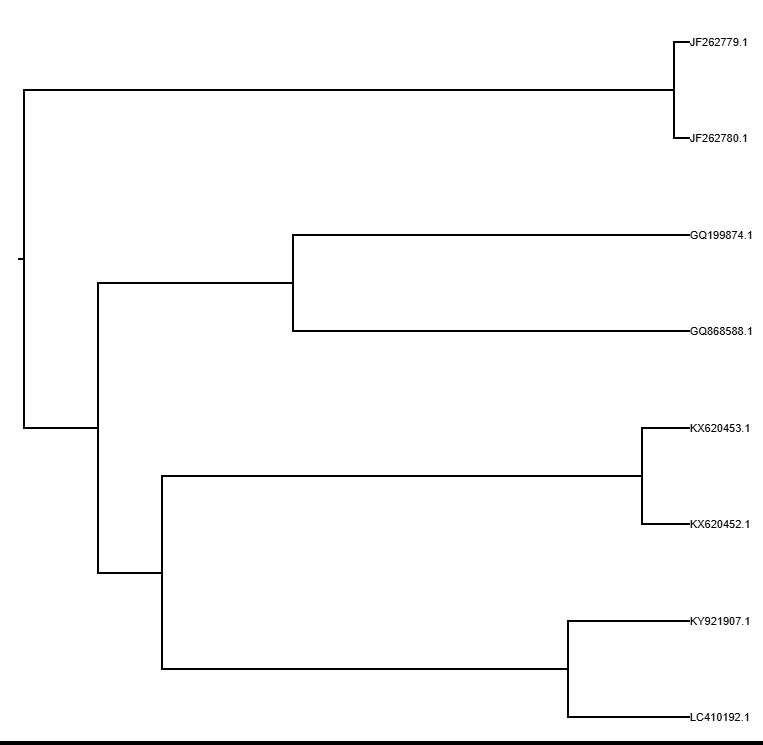
\includegraphics[width=\textwidth]{figures/euclidean_original.jpeg}
    \caption{Euclidean Distance Newick Tree of the original subtypes}
\end{figure}

\begin{figure}[htbp]
    \centering
    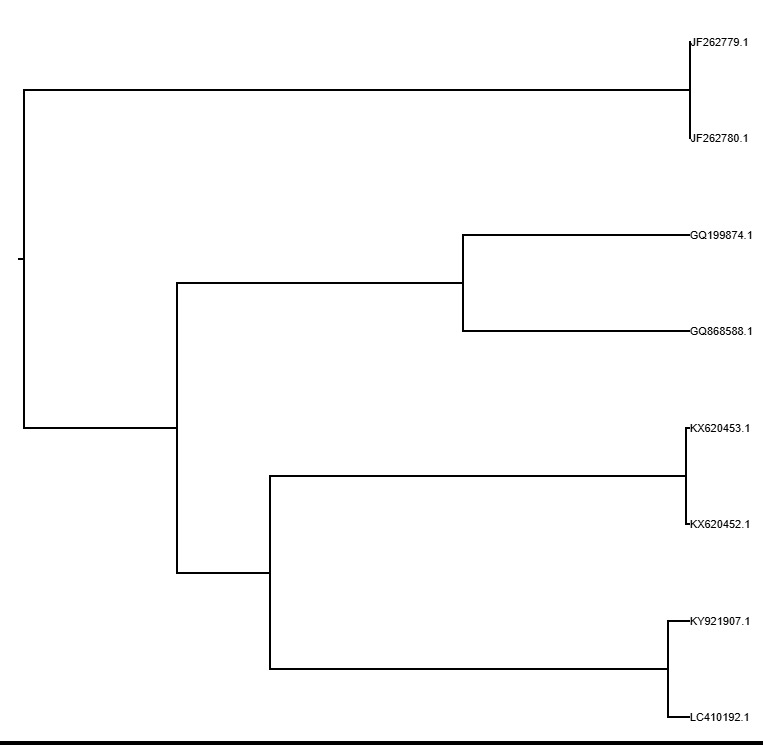
\includegraphics[width=\textwidth]{figures/cosine_original.jpeg}
    \caption{Cosine Similarity Newick Tree of the original subtypes}
\end{figure}

\begin{figure}[htbp]
    \centering
    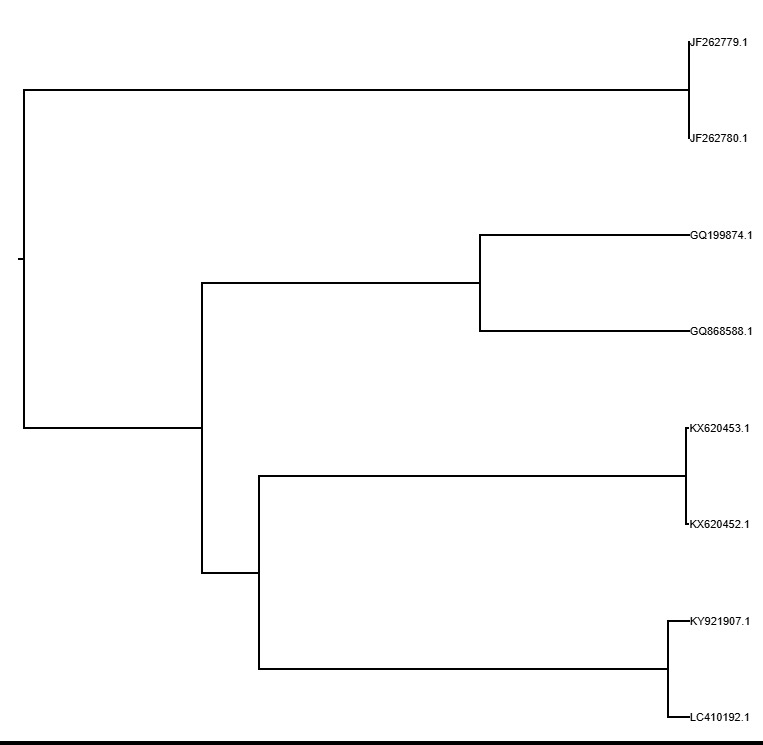
\includegraphics[width=\textwidth]{figures/pearson_original.jpeg}
    \caption{Pearson Correlation of Newick Tree of the original subtypes}
\end{figure}
\newpage

\subsection*{Test Sequence}
With the test sequence, we see a slight change in the tree, where we simply add sequence 9 in.

\begin{figure}[htbp]
  \centering
    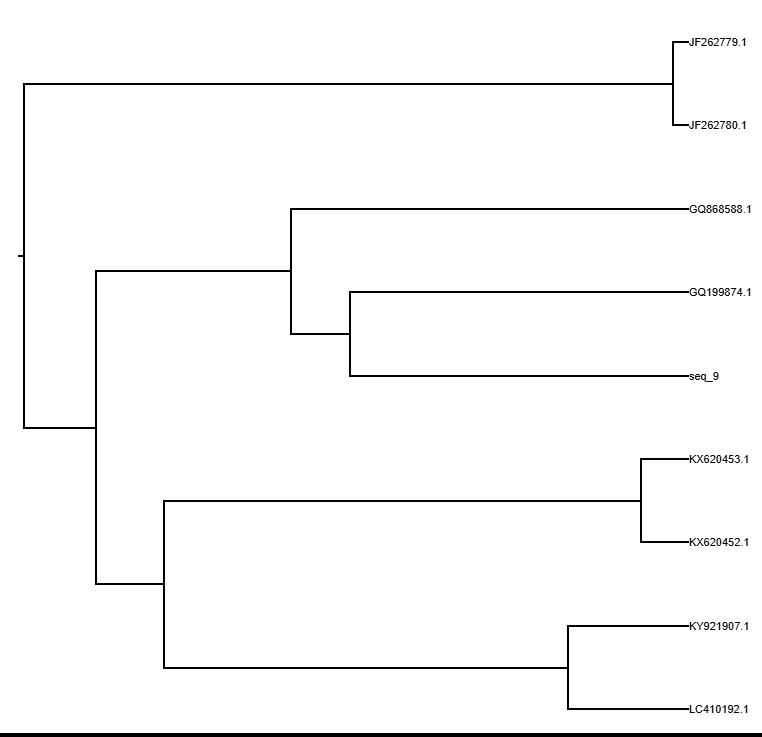
\includegraphics[width=\textwidth]{figures/euclidean_candidate.jpeg}
    \caption{Euclidean Distance Newick Tree with the test sample}
\end{figure}

\begin{figure}[htbp]
    \centering
    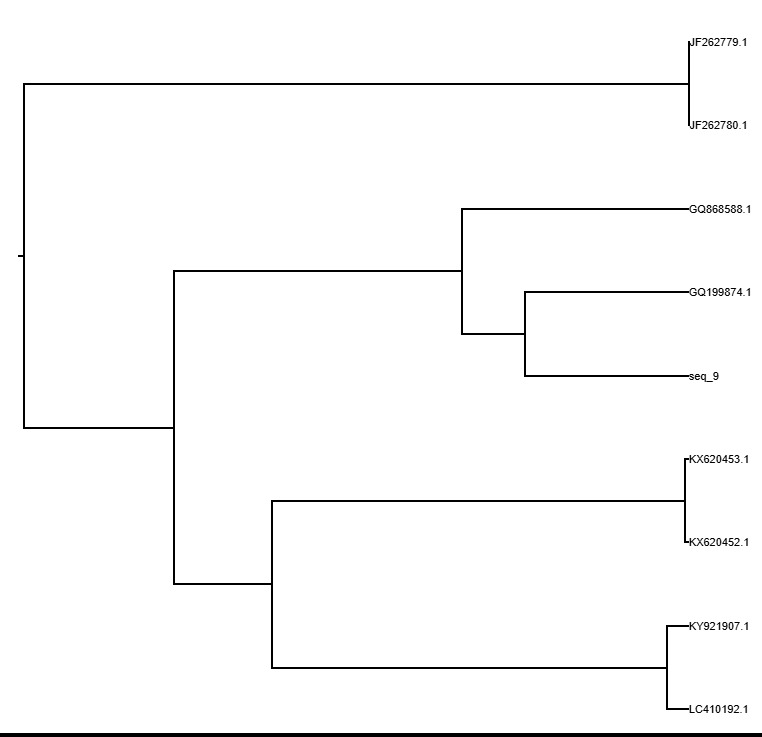
\includegraphics[width=\textwidth]{figures/cosine_candidate.jpeg}
    \caption{Cosine Similarity Newick Tree with the test sample}
\end{figure}

\begin{figure}[htbp]
    \centering
    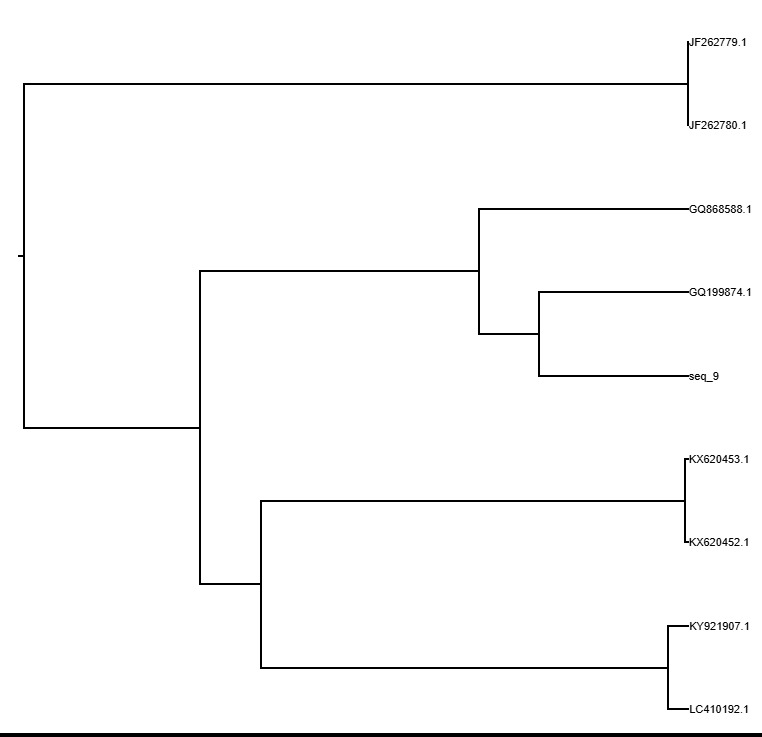
\includegraphics[width=\textwidth]{figures/pearson_candidate.jpeg}
    \caption{Pearson Correlation of Newick Tree with the test sample}
\end{figure}
\newpage
\subsection*{Predicted subtype}
In all cases, we have that our subtype sequence 9 belongs to subtype2, and is a sibling of GQ199874.1.

\subsection*{Appropriate Metric}
In my opinion, I believe that cosine similarity to be the best metric as it is the most interpretable and grounded in what we want.\\

For Euclidean distance, a problem arises if we have two sequence frequencies of $[0, 1]$ and $[0, 2]$. If the direction is the same for the vectors, as it is here, then we know that the relative frequencies of the kmers are the same and therefore should not be penalized. However, for Euclidean distances, this is penalized.\\

Now, we can note that this is not penalized in both cosine similarity and Pearson correlation. For cosine similarity this is because the two vectors are in the exact same direction. For Pearson correlation this is because the correlation between the variables matches. In fact, one can show that my metrics I've used have the same derivative and grows at the same rate as each other. i.e. for any change in Pearson correlation distance metric, we would expect similar changes in the cosine similarity distance metric. In fact, looking at the previous figures, there is very little discrepancy between the two models. Therefore this boils down to how interpretable the two metrics are.\\

I argue that the cosine similarity is a more interpretable metric. Cosine similarity simply measures the angle between two vectors. This therefore measures the relative changes in components of both vectors. For frequency, we can imagine that this means how much the relative frequency matches with each other. This relative frequency can then be used as a heuristic for how similar two species are.\\

However, for the Pearson correlation, we are assuming that the various frequencies act essentially as independent samples of a distribution that might be correlated with another distribution. It is not exactly clear what $\rho = 0$ and its difference from $\rho = -1$, and how much this negative correlation should be taken into account as dissimilarity.\\

Therefore for its interpretability and usage as a metric, I believe that the cosine similarity should be the best metric to use.

\section*{Part 4: Genome Assembly}
All code and examples are found under `q4/'. This problem was tackled with the following strategy:
\begin{enumerate}
  \item Grab the sequences and create an aggregate kmer-frequency array of length kmer by summing up the frequency over all possible kmers.
  \item With the optional flag `-t' or `--tol', allow the user to define what kmer frequency should be merged with its neighbours, defined as all possible kmers that are a single nucloetide away. This is the error correction step.
  \item Generate the deBrujin graph based on the total frequency of kmers by simply grabbing each kmer and setting the from kmer as the prefix and the to kmer as the suffix.
  \item Do some analysis on this graph, including finding all the components. From these components, remove all components except for the largest one. Empirically, most of these components should be safe to remove; with kmer of size 9, we see that the component sizes are $\{7679, 2, 2, 6, 2, 3, 3, 2\}$. Since these are small enough and would potentially cause deadends within the Eulerian path finding, we remove them.
  \item Next, we clean the graph optionally using the `--clean$\_$graph' flag which if used will add and remove potential edges that are making certain nodes' indegrees and outdegrees unbalanced. Given more time, I would have added the marking of a node's depth and the removal of any branches that lead nowhere.
  \item Finally, we find the Eulerian path (or a close one) by traversing over the edges randomly until we cannot anymore. Note this was done by turning the number of edges into weights for a probability distribution. For the starting point, we choose the node with the most out going edges compared to the incoming edges as this is more likely to be the true starting sequence.
\end{enumerate}

Run the code with the following: `python assemble$\_$genome.py -i $<$input$\_$file$>$' with the following optional flags:
\begin{enumerate}
  \item `--output$\_$dir' specifies the output directory. If set, this also changes the output file to be of form: $<$input$>\_$assembled$\_$genome$\_$kmer$\_<$kmer-length$>\_$tol$\_<$tolerance$>\_$clean$\_$graph$\_<$clean-graph$>\_$seed$\_<$seed$>$.fna
  \item `--kmer$\_$len' specifies the kmer length to be used. Note that this makes the runtime exponentially slower due to the frequency array analysis. From experience, anything beyond $k=10$ might be unbearable, and not worth it; see the k-mer length ablations section.
  \item `--tol' specifies the upper bound for where we will move the kmer frequencies from one variable to another. See the error correction step ablations section for more details.
  \item `--clean$\_$graph' is a boolean flag which if set to true will add edges from some nodes to others and remove them where possible to balance the tree more. More details found under cleaning graph ablations.
  \item `--seed'. \textbf{Note: This at the moment seems to be broken and cannot recover the same nucleotide sequence. So, my best run using $k = 10$ may or may not be replicable, depending on how lucky one is}.
\end{enumerate}

For one of my best runs, I used the k-mer length of 10, the tolerance set to 1, the seed set to 42 and setting the graph cleaning to true.

\newpage

\subsection*{BLAST Testing}
For BLAST testing, I simply tested against the \href{https://blast.ncbi.nlm.nih.gov/Blast.cgi?PROGRAM=blastn&PAGE_TYPE=BlastSearch&LINK_LOC=blasthome}{BLAST website}. This will be a verification alongside other heuristics for how good alignments are alongside how certain ablations led to better results.\\

For my results, I predict that the virus is of HIV strand, by the following output from BLAST after running on my file with the setting described above. Specifically, it might be \textit{PQ511694.1} according to total score:
\begin{figure}[htbp]
    \centering
    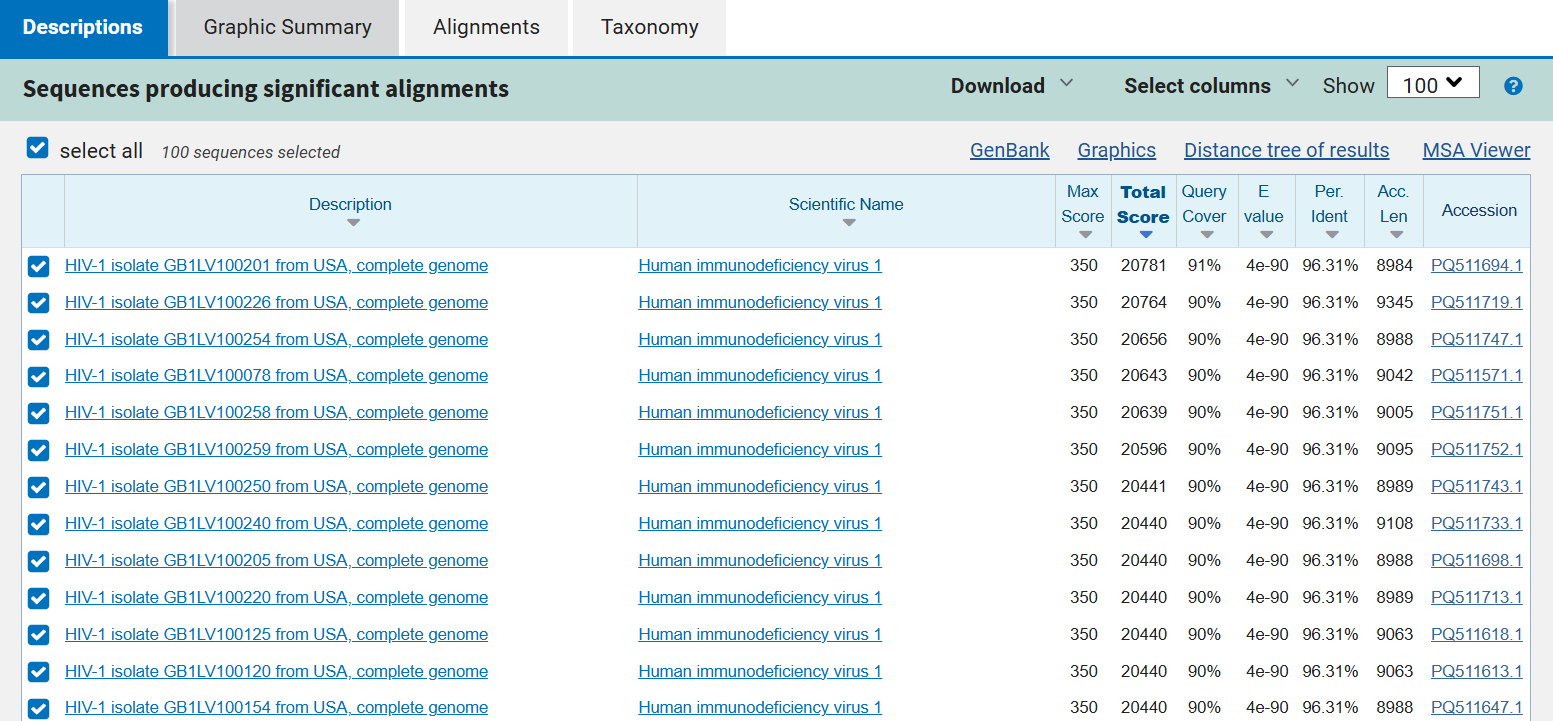
\includegraphics[width=\textwidth]{figures/blast_output_k_10.PNG}
    \caption{BLAST Output with viral alignments}
    \label{fig:figure_7}
\end{figure}

\subsection*{Error Correction Step Ablations}
For this set of ablations, I looked at understanding how the tolerance flag will help or reduce the accuracy of the alignment. These ablations might not be entirely accurate because the seeding is not working properly and we would want to average over multiple seeds. However, it still showcases the general trends we would want to look to for building an understanding on how this hyperparameter affects the results.\\

Below is a table of the resultant number of nodes, edges and components, assembled sequence based on different tolerances for $k=9$:\\
\begin{table}[h]
\centering
\begin{tabular}{c|ccc}
Tolerance & 0 & 1 & 2 \\ \hline
Node Count & 8261 & 7699 & 7666 \\
\hline
Edge Count & 82770 & 82770 & 82770 \\
\hline
Component Count & 1 & 8 & 21\\
\hline
Sequence length & 5973 & 2040 & 8
\end{tabular}
\caption{Graph Analysis on Various Tolerance Ablations}
\label{tab:table_1}
\end{table}

Generally, there are less nodes (with the same number of edges as expected) but a higher number of components due to cutting off the bridges between components. This however, is not an issue because each component is composed of a very small number of kmers, meaning that they are likely to be errors than anything else. Switching these reads to an existing read is a much more likely situation.\\

However, careful consideration is needed as with this run, if you use tolerance as 2, the resultant sequence length gets reduced down to 8 nucleotides a piece, likely due to a higher frequency of edges going towards a short branch, and being unlucky and getting stuck. This can be resolved through graph cleaning, and pruning any of these short branches.

\subsection*{K-mer Length Ablations}
The k-mer length is probably the most important hyperparameter in this code, as it determines the graph structure and how well this graph structure will be traversed.\\

The following table showcases the ablations done on the k-mer length, uncovering how the graph changes over time, and the resultant downstream effect on the assembled genome sequence length given the same starting seed. The results can be seen under the `logs/' folder, and can be executed by running the `run$\_$k$\_$ablations.sh' bash script.
\begin{table}[h]
\centering
\begin{tabular}{c|ccccccccc}
k-mer length & 2 & 3 & 4 & 5 & 6 & 7 & 8 & 9 & 10 \\ \hline
Node Count & 4 & 16 & 64 & 255 & 937 & 2840 & 5655 & 7699 & 8607\\
\hline
Edge Count (before cleaning) & 89000 & 88110 & 87220 & 86330 & 85440 & 84550 & 83660 & 82770 & 81880 \\
\hline
Component Count & 1 & 1 & 1 & 1 & 1 & 2 & 6 & 8 & 10\\
\hline
Degree average (before cleaning) & 23 & 7.75 & 2.94 & 1.87 & 0.958 & 0.562 & 0.368 & 0.282 & 0.228\\
\hline
Degree average (after cleaning) & 0 & 3.125 & 1.19 & 0.48 & 0.303 & 0.218 & 0.195 & 0.170 & 0.166 \\
\hline
Outdegree average (after cleaning) & 22261.5 & 5506.5 & 1363.3 & 338.88 & 91.354 & 29.891 & 14.868 & 10.8 & 9.56 \\
\hline
Sequence length (after cleaning) & 89042 & 87706 & 85999 & 74742 & 76020 & 39537 & 8395 & 2042 & 11669
\end{tabular}
\caption{K-mer Length effect on graph counts for tolerance of 1}
\end{table}

Note the degree average refers to taking the absolute value of the difference between the indegree and outdegree and averaging this over all the nodes. This was repeated for before graph cleaning (adding or removing edges) and after it.\\

As for the results, first note the sequence length as $k$ increases. Note that at the start, they are taking every single edge possible due to the low-complexity of the graph, meaning that it is utilizing the k-mers as well as possible. This however comes at the cost of it being highly inaccurate; if it can take any route possible, then it is simply relying on luck to know how to assemble the genome. As an aside: the sequence length can be larger than the edge count due to counting the edges before cleaning, and cleaning might lead to some extra edges added.\\

This generally means that as $k$ increases, and the outdegree average decreases, that we are choosing better and better paths due to being more confident that if an edge exists, that it should exist in the original sequence. However, we run into issues where it is more likely to get stuck, as showcased in \hyperref[tab:table_1]{Table 1}'s tolerance of 2 result, causing sequences that are too short. This can be fixed by graph cleaning and pruning to get rid of branches that are too short.\\

However, this does not necessitate that longer is worse for my code, in fact on one lucky seed for $k=10$, we managed to get a sequence length of 11669, with a high score of \hyperref[fig:figure_7]{20781}.

\subsection*{Cleaning Graph Ablations}
It is still uncertain whether my graph cleaning is helpful as running BLAST resulted in no significant increase or decrease in score between cleaning ablations. However, based on heurisitcs, we can assume that this graph cleaning does help as we manage to increase the chances of continuing the path finding. This holds because the degree average after cleaning decreases across all $k$, meaning that it approximates a graph with a Euclidean cycle much better. However, it is important to note that the usefulness decreases as $k$ increases, as the difference in the average after cleaning starts to decrease.

\newpage
\subsection*{Future Extensions}
In the future, I wish to add the following:
\begin{enumerate}
  \item Graph cleaning and pruning to get rid of branches that are too short. This can be done through calculating the dfs path to a leaf and removing the ones that are not within a cycle.
  \item Proper seeding so that experiments are repeatable and results are verifiable. Also, re-running these ablations on multiple different seeds.
  \item Support higher values of $k$ by using sparse methods instead of building the $4^k$ frequency array.
\end{enumerate}

\end{document}
